\documentclass[10pt]{article}
\usepackage[utf8]{inputenc}
\usepackage{mathtools}
\usepackage{amsmath}
\usepackage{graphicx}
\usepackage{array}
\usepackage[margin=0.5in]{geometry}
\usepackage{listings}
\usepackage{color}

\definecolor{mygreen}{rgb}{0,0.6,0}
\definecolor{mygray}{rgb}{0.5,0.5,0.5}
\definecolor{mymauve}{rgb}{0.58,0,0.82}

\lstset{ %
  backgroundcolor=\color{white},   % choose the background color; you must add \usepackage{color} or \usepackage{xcolor}; should come as last argument
  basicstyle=\footnotesize,        % the size of the fonts that are used for the code
  breakatwhitespace=false,         % sets if automatic breaks should only happen at whitespace
  breaklines=true,                 % sets automatic line breaking
  captionpos=b,                    % sets the caption-position to bottom
  commentstyle=\color{mygreen},    % comment style
  deletekeywords={...},            % if you want to delete keywords from the given language
  escapeinside={\%*}{*)},          % if you want to add LaTeX within your code
  extendedchars=true,              % lets you use non-ASCII characters; for 8-bits encodings only, does not work with UTF-8
  frame=single,	                   % adds a frame around the code
  keepspaces=true,                 % keeps spaces in text, useful for keeping indentation of code (possibly needs columns=flexible)
  keywordstyle=\color{blue},       % keyword style
  language=Octave,                 % the language of the code
  morekeywords={*,...},            % if you want to add more keywords to the set
  numbers=left,                    % where to put the line-numbers; possible values are (none, left, right)
  numbersep=5pt,                   % how far the line-numbers are from the code
  numberstyle=\tiny\color{mygray}, % the style that is used for the line-numbers
  rulecolor=\color{black},         % if not set, the frame-color may be changed on line-breaks within not-black text (e.g. comments (green here))
  showspaces=false,                % show spaces everywhere adding particular underscores; it overrides 'showstringspaces'
  showstringspaces=false,          % underline spaces within strings only
  showtabs=false,                  % show tabs within strings adding particular underscores
  stepnumber=2,                    % the step between two line-numbers. If it's 1, each line will be numbered
  stringstyle=\color{mymauve},     % string literal style
  tabsize=2,	                   % sets default tabsize to 2 spaces
  title=\lstname                   % show the filename of files included with \lstinputlisting; also try caption instead of title
}
\renewcommand{\arraystretch}{1.5}
\setcounter{secnumdepth}{0}
\author{Kevin Mambu}
\date{\today}
\title{M1 SESI 2017-2018\\Architecture Multi-Processeurs\\TP7 : Contrôleur DMA}

\begin{document}
\maketitle

\section{A) Objectifs}
Le but de ce TP est d’analyser le fonctionnement d'un périphérique plus complexe
que ceux analysés dans le TP6. Un périphérique possédant une capacité DMA
(Direct Memory Access) se comporte à la fois comme un maître capable de lire ou
d'écrire directement en mémoire, et comme une cible capable - comme n'importe
quel périphérique - de recevoir des commandes provenant du système
d'exploitation.

On utilise la même architecture que dans le TP5 et le TP6, mais on instanciera
un seul processeur, et on activera le contrôleur DMA. On utilisera des caches
possédant une capacité de 2 Koctets (lignes de 16 octets, 4 niveaux
d'associativité, 32 sets).

\section{B) Contrôleur DMA}
\begin{center}
  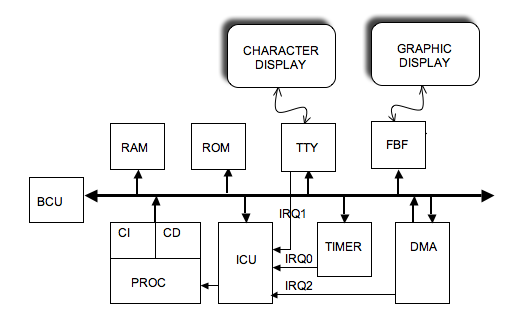
\includegraphics[width=9cm]{tp7_topcell_dma.png}
\end{center}

\subsection{Question B1}
\begin{tabular}{|c|c|p{5cm}|}
  \hline
  \multicolumn{3}{|c|}{Registres adressables du contrôleur DMA}\\ \hline
  \texttt{SOURCE} & 0x00 (RW) & Adresse de base du tampon source \\ \hline
  \texttt{DEST} & 0x04 (RW) & Adresse de base du tampon destinataire \\ \hline
  \texttt{NWORDS/STATUS} & 0x08 (RW) &  \begin{itemize}
                                          \item si écriture $\rightarrow$
                                          démarre un transfert DMA pour le
                                          nombre de mots spécifié.
                                          \item si lecture $\rightarrow$
                                          contient le statut de retour du
                                          transfert DMA :
                                          \begin{itemize}
                                            \item DMA\_IDLE
                                            \item DMA\_SUCCESS
                                            \item DMA\_READ\_ERROR
                                            \item DMA\_WRITE\_ERROR
                                          \end{itemize}
                                        \end{itemize} \\ \hline
  \texttt{RESET} & 0x0C (R) & Reset logiciel, écrire dans ce registre pour
                              acquitter l'interruption du contrôleur DMA. \\ \hline
  \texttt{IRQ\_DISABLED} & 0x10 (RW) & IRQ désactivée si $\neq0$ \\ \hline
\end{tabular}
\begin{itemize}
  \item L’adresse de base du segment associé au contrôleur DMA en tant que cible
  doit être alignée sur une frontière de bloc de 32 octets par souci
  d'alignement (segment de 32 octets).
\end{itemize}

\subsection{Question B2}
\texttt{burst} est l'argument permettant de spécifier le nombre maximal de mots
qui peuvent être transferés lors d'une rafale (\textit{Burst}).

\subsection{Question B3}
Le coprocesseur DMA requiert deux automates MASTER\_FSM et TARGET\_FSM afin de
pouvoir :
\begin{itemize}
  \item Recevoir des commandes d'autres maîtres (en qualité de cible).
  \item Initier des transactions mémoires (en qualité de maître).
\end{itemize}
Ces deux tâches doivent pouvoir se faire simultanément.

\subsection{Question B4}
La bascule \texttt{r\_stop} est une bascule commandée par l'automate
TARGET\_FSM. Elle est en popsition basse lors d'un transfert DMA (e.g. lorsque
MASTER\_FSM est à l'état DMA\_IDLE) et est positionnée à true à la fin d'un
transfert DMA par le bais du registre RESET.

\subsection{Question B5}
\begin{center}
  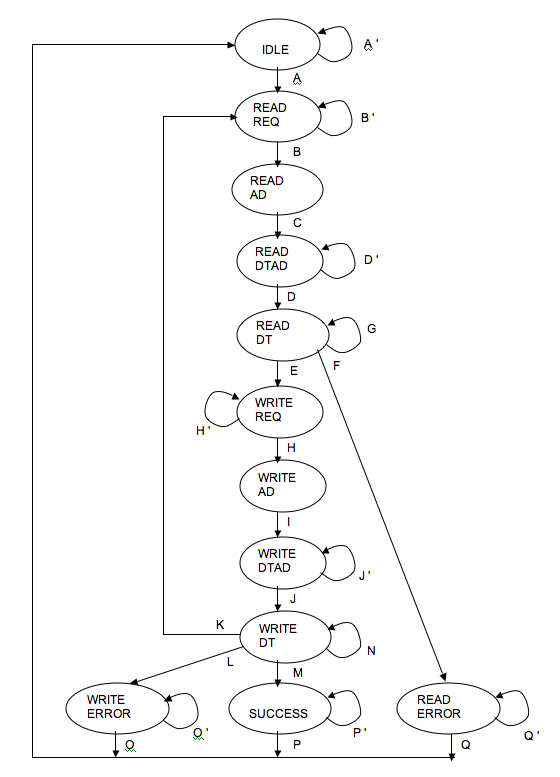
\includegraphics[width=9cm]{tp7_master_fsm.png}
  \begin{tabular}{|c|c|}
    \hline
    \multicolumn{2}{|c|}{Transitions de MASTER\_FSM} \\ \hline
    A'  & $\overline{R\_STOP}$ \\ \hline
    A   & $R\_STOP$ \\ \hline
    B'  & $\overline{GNT}$ \\ \hline
    B   & $GNT$ \\ \hline
    C   & $true$ \\ \hline
    D'  & $WAIT$ \\ \hline
    D   & $\overline{WAIT}$ \\ \hline
    E'\footnote[1] & $\overline{ERROR}\bullet{READY}\bullet{R\_STOP}$ \\ \hline
    E   & $\overline{ERROR}\bullet{READY}\bullet\overline{R\_STOP}$ \\ \hline
    F   & $ERROR$ \\ \hline
    G   & $\overline{READY}+\overline{ERROR}$ \\ \hline
    H'  & $\overline{READ}$ \\ \hline
    H   & $READ$ \\ \hline
    I   & $true$ \\ \hline
    J'  & $\overline{READY}$ \\ \hline
    J   & $READY$ \\ \hline
    K'\footnote[1] & $\overline{ERROR}\bullet{READY}\bullet{R\_STOP}$ \\ \hline
    K   & $\overline{ERROR}\bullet{READY}\bullet\overline{R\_STOP}\bullet{R\_COUNT}$ \\ \hline
    L   & ${ERROR}$ \\ \hline
    M   & $\overline{ERROR}\bullet{READY}\bullet\overline{R\_STOP}\bullet\overline{R\_COUNT}$ \\ \hline
    N   & $\overline{READY}+\overline{ERROR}$ \\ \hline
    O', P', Q' & $\overline{R\_STOP}$ \\ \hline
    O, P, Q & $R\_STOP$ \\ \hline
  \end{tabular}
\end{center}

\texttt{[1]} : Ces transitions n'apparaissent pas sur le graphe du sujet, mais
servent de point de retour en cas d'erreur : si le maître responsable de la
transaction se fait tué avant la fin de cette dernière, le contrôleur DMA
avorte alors son transfert puis retourne dans l'état IDLE. {\bf Uniquement à
la fin d'un transfert sur le PIBUS (XXX\_DT), sinon ce dernier se retrouverait
bloqué!}

\section{C) Architecture matérielle}

\subsection{Question C1}

\begin{itemize}
  \item Par défault, la longeur d'une rafale de mots 32 bits est de 16 mots.
  \item Utiliser de grosses rafales permet de réduire le nombre de réquisitions
  du Pibus, plusieurs mots tranferés pour une réquisition du bus.
  \item Dans la description \textit{\texttt{pibus\_dma.cpp}}, on peut voir que
  le \texttt{burst} est borné entre 0 et 128. Augmenter la longeur maximale
  d'une rafale augmenterait la taille des tampons internes du périphérique DMA.
\end{itemize}
\subsection{Question C2}
\begin{itemize}
  \item L'adresse de base du segment associé au périphérique DMA est
  \texttt{0x93000000}.
  \item L'index de cible vis-à-vis du BCU est \texttt{DMA\_INDEX}, égal à 6.
  \item Son numéro de maître est à \texttt{nprocs + 1}. Sur notre, architecture
  mono-processeur, son index de maître est alors à 2.
  \item La ligne d'interruption IRQ contrôlée par le périphérique DMA est relié
  au port d'entrée IRQ\_IN[0] du composant ICU.
\end{itemize}

\section{D) Application logicielle}
\subsection{Question D1}
\begin{itemize}
  \item Lors de la fonction fb\_sync\_write, le processeur exécutant cette
  fonction est à la charge de l'écriture du tampon dans le segment réservé
  au FrameBuffer, par l'intermédiaire du appel système.
  \item Cet appel est alors naturellement bloquant car, rappelons le, parmi
  les requêtes d'accès mémoire, les écritures en Tampon d'Écriture Postées sont
  les plus prioritaires et la donnée à écrire l'est dans un segment non-cachable.
\end{itemize}

\subsection{Question D2}
\begin{center}
  \begin{tabular}{|c|c|c|c|c|c|c|}
    \hline
     & Damier 5 & Damier 4 & Damier 3 & Damier 2 & Damier 1 & Moyenne \\ \hline
     Display (cy) & 117148 & 117161 & 117161 & 117175 & 117353 & 117200 \\ \hline
     Build (cy) & 717883 & 713813 & 717827 & 717822 & N.C. & 716837 \\ \hline
  \end{tabular}
\end{center}

\subsection{Question D3}

La fonction fb\_sync\_write() force une attente active jusqu'à la fin de
l'écriture vers le FrameBuffer tandis que fb\_write() déclenche l'écriture de
manière non-bloquante, via le coprocesseur DMA. La vérification de la fin du
transfert se fait grâce à la fonction fb\_completed().

\subsection{Question D4}
\begin{center}
  \begin{tabular}{|c|c|c|c|c|c|c|}
    \hline
     & Damier 5 & Damier 4 & Damier 3 & Damier 2 & Damier 1 & Moyenne \\ \hline
     Display (cy) & 4199 & 4199 & 4199 & 4260 & 4036 & 4179 \\ \hline
  \end{tabular}
\end{center}

\subsection{Question D5}
Sur le bord gauche de l'image affichée, on peut observer une portion de cases
appartenant au damier de l'itération suivante. Cela est dû au fait que faute
de synchronisation sur la bonne écriture du buffer, les premières cases du
buffer ont le temps d'être écrasées avant d'être envoyées au FrameBuffer.

\subsection{Question D6}
\begin{itemize}
  \item
  \begin{itemize}
    \item Dans \_fb\_completed(), tant que la variable \_dma\_busy est
    différente de 0, le processeur est bloqué.
    \item Dans \_fb\_write(), tant que \_dma\_busy est différente de 0, le
    processeur attend une période pseudo-aléatoire, une fois que \_dma\_busy est
    égale à 0, le processeur la remet à 1.
  \end{itemize}
  \item La routine d'interruption \_isr\_dma est la fonction qui remet à 0 le
  flag \_dma\_busy.
  \item Le vecteur de flags \texttt{\_dma\_busy} est stocké dans le segment
  seg\_unckdata.
\end{itemize}

\section{E) Pipe-line logiciel}

\subsection{Question E1}
Pour pouvoir passer de la période (n) à la période (n+1), il faut que le
transfert du DMA au Framebuffer soit terminé à la période (n). Nous utiliserons
la fonction \_fb\_completed.

\subsection{Question E2}
\begin{center}
  \begin{tabular}{|c|c|c|c|c|c|c|}
    \hline
     & Damier 5 & Damier 4 & Damier 3 & Damier 2 & Damier 1 & Moyenne \\ \hline
     Display (cy) & 3979 & 4086 & 3984 & 4240 & 3690 & 3996 \\ \hline
     Build (cy) & 716739 & 716789 & 716901 & 716871 & N.C. & 716825 \\ \hline
  \end{tabular}
\end{center}

\begin{itemize}
  \item Le gain apporté par le parallelisme pipeline par rapport à une
  exécution séquentielle est de 183 cycles, ce qui est bien maîgre gain
  comparé au coût de l'implémentation (ajout d'un if, ajout d'un tampon).
  \item Ce chiffre est significatif d'une chose : le temps de construction d'un
  damier est négligeable par face au temps de transfert d'un damier via le
  contrôleur DMA.
\end{itemize}

\section{F) Traitement des erreurs}

\subsection{Question F1}
fb\_read() et fb\_write() sont des fonctions qui font des accès mémoire, en ce
sens il ne faut pas que le tampon source ou destination soit de la zone mémoire
privilégiée :
\begin{itemize}
  \item fb\_read() a la possibilité de permettre de l'injection de données dans
  le système d'exploitation.
  \item fb\_write() a la possibilité de dévoiler des portions de l'espace
  système auquel l'utilisateur ne devrait pas avoir accès.
\end{itemize}

Une fois la requête envoyée au contrôleur DMA, plus aucun contrôle de droits ou
de sécurité n'est effectué. Cette vérification doit être fait a priori.

\subsection{Question F2}
\begin{itemize}
  \item À l'échelle du composant Pibus\_DMA, en cas d'erreur le composant passe
  dans l'état DMA\_XXXXX\_ERROR, puis lève une interruption.
  \item À l'échelle de la routine \_isr\_dma, la routine sauvegarde dans le
  registre \_dma\_status la cause de la levée d'interruption.
  \item À l'échelle de \_fb\_completed(), si le \_dma\_status est différent de
  0, la fonction retourne 1 (cas d'erreur).
\end{itemize}

\subsection{Question F3}
\begin{itemize}
  \item fb\_sync\_write
  \begin{itemize}
    \item sys\_call(FB\_SYNC\_WRITE...
    \item syscall
    \item \_fb\_write(...
    \item C'est dans la fonction de driver que la vérification des
    arguments se fait :\\
  \end{itemize}
\end{itemize}
\begin{lstlisting}
  if (((unsigned int) buffer >= 0x80000000)
    || (((unsigned int)buffer + length) >= 0x80000000) )
    return 1;
\end{lstlisting}

\newpage

\lstinputlisting[language=C]{./main_pipe.c}
\end{document}
